%%%%%%%%%%%%%%%%%%%%%%%%%%%%%%%%%%%%%%%%%
% fphw Assignment
% LaTeX Template
% Version 1.0 (27/04/2019)
%
% This template originates from:
% https://www.LaTeXTemplates.com
%
% Authors:
% Class by Felipe Portales-Oliva (f.portales.oliva@gmail.com) with template 
% content and modifications by Vel (vel@LaTeXTemplates.com)
%
% Template (this file) License:
% CC BY-NC-SA 3.0 (http://creativecommons.org/licenses/by-nc-sa/3.0/)
%
%%%%%%%%%%%%%%%%%%%%%%%%%%%%%%%%%%%%%%%%%

%----------------------------------------------------------------------------------------
%	PACKAGES AND OTHER DOCUMENT CONFIGURATIONS
%----------------------------------------------------------------------------------------

\documentclass[
	english,
	11pt, % Default font size, values between 10pt-12pt are allowed
	%letterpaper, % Uncomment for US letter paper size
	%spanish, % Uncomment for Spanish
]{fphw}

% Template-specific packages
\usepackage{babel}
\usepackage[utf8]{inputenc} % Required for inputting international characters
\usepackage[T1]{fontenc} % Output font encoding for international characters
\usepackage{mathpazo} % Use the Palatino font
% \usepackage{iwona} % Use the Iwona font

\usepackage{amsmath}
\usepackage{mathtools}
\usepackage{cases}	% Required to use nmbered tags in cases

\usepackage{graphicx} % Required for including images
\usepackage{caption}  %% To manage long captions in images
\usepackage{subcaption}
\usepackage{float}
\graphicspath{ {./img/} }

\usepackage{booktabs} % Required for better horizontal rules in tables

\usepackage{listings} % Required for insertion of code

\usepackage{array} % Required for spacing in tabular environment

\usepackage{enumerate} % To modify the enumerate environment

\usepackage{amssymb}
\usepackage{enumitem}	%% % To modify the itemize bullet character

\usepackage[linkcolor=blue,colorlinks=true]{hyperref}
\usepackage{cleveref}  %% To make links clickable

\newcommand{\hquad}{\hspace{0.5em}} %% Bew command for half quad
\usepackage{indentfirst}	%% Indent the first paragraph
\newcommand{\bi}{\text{Bi}} 


%----------------------------------------------------------------------------------------
%	ASSIGNMENT INFORMATION
%----------------------------------------------------------------------------------------

\title{Problem Set \#1: RB for Linear Affine Elliptic} % Assignment title

\author{Roussel Desmond Nzoyem} % Student name

\date{\today} % Due date

\institute{University of Strasbourg \\ UFR de Mathématiques et Informatique} % Institute or school name

\class{Calcul Scientifique 3} % Course or class name

\professor{Pr. Christophe Prud'homme} % Professor or teacher in charge of the assignment

%----------------------------------------------------------------------------------------

\begin{document}

\maketitle % Output the assignment title, created automatically using the information in the custom commands above

%----------------------------------------------------------------------------------------
%	ASSIGNMENT CONTENT - SECTION 1
%----------------------------------------------------------------------------------------


\section{Part 1 - Finite Element Approximation}

\subsection*{Question a)}
\begin{problem}
	Let's show that $u^e(\mu) \in X^e \equiv H^1(\Omega)$ satififies the weak form.
	\begin{equation}
		\tag{7}\label{eq:7}
		a(u^e(\mu),v;\mu)=l(v), \quad \forall v \in X^e 
	\end{equation}

	with
	$$
		a(w,v;\mu) = \sum_{i=0}^{4} k^i \int_{\Omega_i} \nabla w \cdot \nabla v \, dA + \bi \int_{\Gamma \\ \Gamma_root} w v \, dS
	$$
	$$
		l(v) = \int_{\Gamma_root} v \, dS
	$$
\end{problem}


\subsection*{Answer} 


\indent Let's start by summarizing the domain names and boundaries. This is done in the picture below.

\begin{figure}[h]
	\centering
	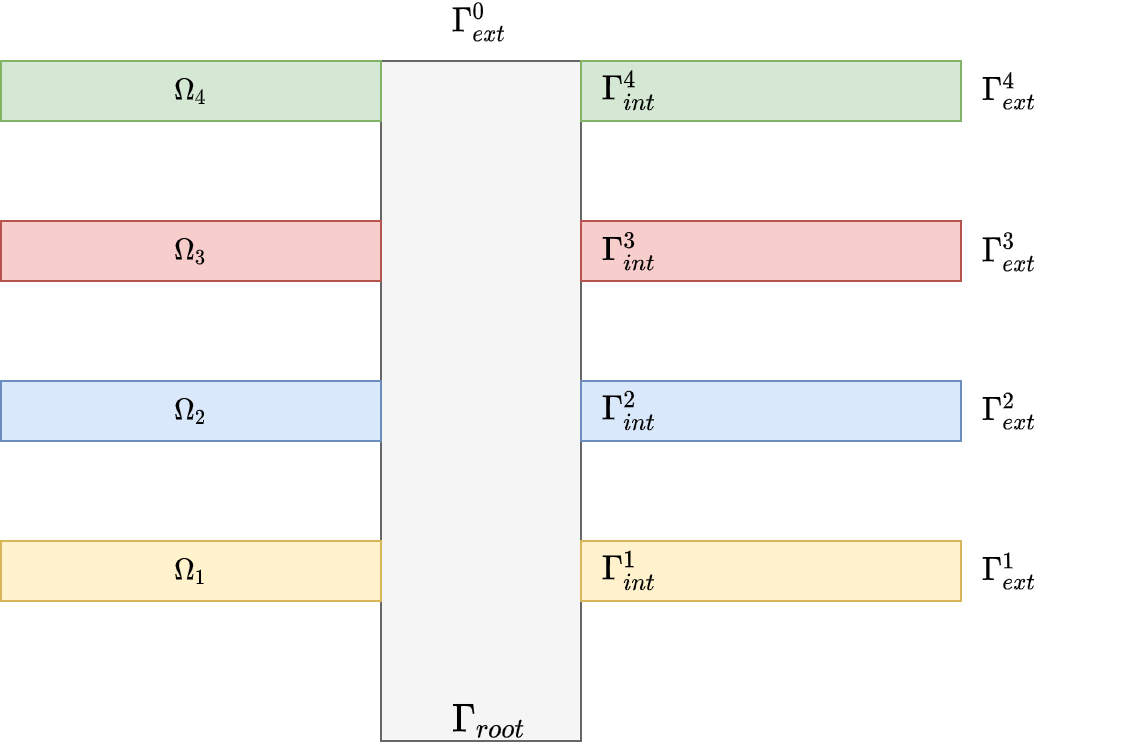
\includegraphics[width=0.6\textwidth]{ThermalFin.png}
	\captionsetup{justification=centering}
	\caption{Domain and boundary denominations for the thermal fin}
\end{figure}

\noindent The thermal heat transfer problem is governed by the following set of equations:

\setcounter{equation}{0}
\begin{numcases}{}
	\hspace*{0.2cm} -k^i \Delta u^i = 0 & $ \quad \text{in} \quad \Omega^i \, , \, i=0,...,4$ \label{eq:1}\\
	\hspace*{0.5cm} u^0 = u^i & $ \quad \text{on} \quad \Gamma_{int}^i \, , \, i=1,...,4$ \label{eq:2}\\
	\hspace*{0.2cm} -(\nabla u^0 \cdot n^i) = -k^i(\nabla u^i \cdot n^i) & $ \quad \text{on} \quad \Gamma_{int}^i \, , \, i=1,...,4$ \label{eq:3}\\
	\hspace*{0.2cm} -(\nabla u^0 \cdot n^0) = -1 & $ \quad \text{on} \quad \Gamma_{root}$ \label{eq:4}\\
	\hspace*{0.2cm} -k^i(\nabla u^i \cdot n^i) = \bi u^i & $ \quad \text{on} \quad \Gamma_{ext}^i \, , \, i=0,...,4$ \label{eq:5}
\end{numcases}

\noindent In the above equation, the parametrized exact solution $u^e(\mu)$ is called $u$ for simplicity. $u^i$ is the restriction of $u$ to $\Omega^i$ with $i = 1,\ldots,4$.

\noindent Using \cref{eq:1}, we get:
\begin{align*}
	&-k^i \Delta u^i = 0 \quad \text{for} \hquad i=0,\ldots,4 \\
	\implies &\int_{\Omega^i}-k^i \Delta u^iv = 0 \quad \forall v \in X^e \quad \text{for} \hquad i=0,\ldots,4
\end{align*}

\noindent Using Green's formula, this yields:
\begin{align} \label{eq:green} \tag{$\ast$}
	\int_{\Omega^i}k^i \nabla u^i \cdot \nabla v - \int_{\partial \Omega^i}k^i \left( \nabla u^i \cdot n^i \right) v  = 0 \quad \forall v \in X^e \quad \text{for} \hquad i=0,\ldots,4
\end{align}

\begin{itemize}
	\item When $i=1,\ldots,4$, we have $\partial\Omega^i = \Gamma_{int}^i \cup \Gamma_{ext}^i$. Using eq. (3) and (5), \eqref{eq:green} becomes:
	$$
	\int_{\Omega^i}k^i \nabla u^i \cdot \nabla v - \int_{\Gamma_{int}^i} \left( \nabla u^0 \cdot n^i \right) v + \bi \int_{\Gamma_{ext}^i} u^i v  = 0 \quad \forall v \in X^e 
	$$
	\item When $i=0$, we have $\partial\Omega^0 = \bigcup_{i=1}^4 \Gamma_{int}^i \cup \Gamma_{ext}^0 \cup \Gamma_{root}$. Using eq. (3), (4), (5) and the fact that $k^0 = 1$, \eqref{eq:green} becomes:
	$$
	\int_{\Omega^0}k^0 \nabla u^0 \cdot \nabla v - \sum_{i=1}^4 \int_{\Gamma_{int}^i} \left( \nabla u^0 \cdot n^0 \right) v + \bi \int_{\Gamma_{ext}^0} u^0 v -\int_{\Gamma_{root}} v  = 0 \quad \forall v \in X^e 
	$$
\end{itemize}

\noindent Now let's perform a summation of \eqref{eq:green} over all the subdomains $\Omega^i, i=0,\ldots,4$.
$$
\sum_{i=0}^4 \int_{\Omega^i}k^i \nabla u^i \cdot \nabla v \underbrace{- \sum_{i=1}^4 \int_{\Gamma_{int}^i}  \left( \nabla u^0 \cdot n^i \right) v - \sum_{i=1}^4 \int_{\Gamma_{int}^i}  \left( \nabla u^0 \cdot n^0 \right) v}_{=\, 0 \text{ because } n^i = -n^0 \text{ on } \Gamma_{int}^i} + \bi \sum_{i=0}^4 \int_{\Gamma_{ext}^i} u^i v -\int_{\Gamma_{root}} v  = 0 \quad \forall v \in X^e 
$$

\noindent Noticing that $\bigcup_{i=0}^4 \Gamma_{ext}^i = \Gamma_{ext} - \Gamma_{root}$, we are left with:
$$
\sum_{i=0}^4 k^i \int_{\Omega^i} \nabla u^i \cdot \nabla v + \bi \int_{\Gamma_{ext} \backslash \Gamma_{root}} u v -\int_{\Gamma_{root}} v  = 0 \quad \forall v \in X^e 
$$

\noindent By writing back $u^e({\mu}) = u$, the above equation can be rewritten as:
$$
\sum_{i=0}^4 k^i \int_{\Omega^i} \nabla u^e({\mu}) \cdot \nabla v + \bi \int_{\Gamma_{ext} \backslash \Gamma_{root}} u^e({\mu}) v = \int_{\Gamma_{root}} v \quad \forall v \in X^e 
$$
We can see that $u^e({\mu})$ satisfies the week form \eqref{eq:7} we set out to prove.


% ---------------------------------------------------------------
% QUESTION 2
% ---------------------------------------------------------------


\subsection*{Question b)}
\begin{problem}
	Let's show that $u^e(\mu)$ is the argument that maximizes.
	\begin{equation}
		\tag{8}\label{eq:J}
		J(w) = \frac{1}{2} \sum_{i=0}^4 k^i \int_{\Omega^i} \nabla w \cdot \nabla w + \frac{\bi}{2} \int_{\Gamma_{ext} \backslash \Gamma_{root}} w^2 -\int_{\Gamma_{root}} w
	\end{equation}
	over all function $w$ in $X^e$.
\end{problem}


\subsection*{Answer} 

As we did in Question a), let's write $u^e(\mu) = u$ to simplify the notations. 

\noindent We need to show that $J(w)>J(u)$ for all $w$ in $X^e$ such that $w \neq u$. 
To that effect, Let's write $w = w + u - u = u + v$ with $v = w-u \in X^e$. 

\noindent For any $w \in X^e$, we have:
\begin{align*}	
J(w) &= J(u+v) \\
&= \frac{1}{2} \sum_{i=0}^4 k^i \int_{\Omega^i} \nabla (u+v) \cdot \nabla (u+v) + \frac{\bi}{2} \int_{\Gamma_{ext} \backslash \Gamma_{root}} (u+v)^2 -\int_{\Gamma_{root}} (u+v) \\ 
&= \frac{1}{2} \sum_{i=0}^4 k^i \int_{\Omega^i} \left( \nabla u \cdot \nabla u + 2 \nabla u \cdot \nabla v + \nabla w \cdot \nabla v\right) + \frac{\bi}{2} \int_{\Gamma_{ext} \backslash \Gamma_{root}} \left( u^2 +2uv+v^2 \right) -\int_{\Gamma_{root}} \left(u + v\right) \\
&= \underbrace{\frac{1}{2}a(u,u; \mu) - l(u)}_{J(u)} + \frac{1}{2}a(v,v;\mu) + \underbrace{a(u,v;\mu)- l(v)}_{0} \\
&= J(u) + a(v,v;\mu) \tag{$\ast$} \label{j}
\end{align*}

Let's show that the bilinear form $a$ is coercive. For any $v \in X^e$ and any parameter $\mu$, we have:
\begin{align*}
	a(v,v;\mu) &= \sum_{i=0}^4 k^i \int_{\Omega^i} \nabla v \cdot \nabla v + \bi \int_{\Gamma_{ext} \backslash \Gamma_{root}} v^2 \\
	&= \sum_{i=0}^4 k^i \int_{\Omega^i} \nabla v \cdot \nabla v + \bi \int_{\Gamma_{ext}} v^2 - \bi \int_{\Gamma_{root}} v^2 \\
	&\geq \underbrace{\min_{0\leq i \leq 4} k^i}_{C_1(\mu)} \int_{\Omega} \nabla v \cdot \nabla v + \bi \int_{\Gamma_{\partial \Omega}} v^2 - \bi \int_{\Gamma_{root}} v^2 \\
	&= C_1(\mu) \left( \lVert \nabla v \rVert_{L^2(\Omega)}^2 +  \frac{\bi}{C_1(\mu)} \lVert v \rVert_{L^2(\partial \Omega)}^2  \right) - \bi \lVert v \rVert_{L^2(\Gamma_{root})}^2 \tag{$\ast \ast$} \label{coercivity}
\end{align*}
Now since $\Omega$ is bounded, open and connected subset of $\mathbb{R}^d$, and $\bi / C_1(\mu) > 0$, a Poincaré-type iniquality (Legoll, 2019, p.48) states there exists a constant $C_2 > 0$ such that 
\begin{align*} \tag{$\ast \ast 1$} \label{poincare}
\forall v \in H^1(\Omega), \hquad \lVert \nabla v \rVert_{L^2(\Omega)}^2 +  \frac{\bi}{C_1(\mu)} \lVert v \rVert_{L^2(\partial \Omega)}^2 \geq C_2 \lVert v \rVert_{H^1(\partial \Omega)}^2
\end{align*} 

\noindent On the other hand, Let's consider the fact that the trace application $\gamma : H^1(\Omega) \rightarrow L^2(\Gamma_{root})$ is continuous, we ca write that :
\begin{align*} \tag{$\ast \ast 2$} \label{trace}
\exists C_3 > 0 \text{ such that }  \lVert v \rVert_{L^2(\Gamma_{root})} \leq C_3 \lVert v \rVert_{H^1(\Omega)}
\end{align*}



\noindent Using the results from \eqref{poincare} and \eqref{trace} , the inequality \eqref{coercivity} leads to:
\begin{align*}
	a(v,v;\mu) \geq C_1(\mu) C_2 \lVert v \rVert_{H^1(\Omega)}^2 - \bi C_3^2 \lVert v \rVert_{H^1(\Omega)}^2
\end{align*}
Finaly, $a$ is coercive since we can write:
$$
a(v,v;\mu) \geq C_4(\mu) \lVert v \rVert_{H^1(\Omega)}^2
$$
with $C_4 = C_1(\mu)C_2-\bi C_3^2$ necessarily $> 0$.

Thanks to this coercivity, we can now return to \cref{j} and see that $J(w) > J(u) = J(u^e(\mu)) \quad \forall w \in H^1(\Omega) = X^e$.Therefore, $u^e(\mu)$ as indicated in \eqref{eq:7} minimizes the functional $J$.





% -------------------------------------------------------------------------------
% REFERENCES
% --------------------------------------------------------------------------------
\section*{References}
\begin{itemize}
	\item Legoll, F. (2019). \textit{Partial Differential Equations and the Finite Element Method}. Retrieved from \href{http://cermics.enpc.fr/~legoll/poly_EDP-EF_jan19.pdf}{this link}.
\end{itemize}

\end{document}
